\documentclass[11pt,a4paper]{article}

\usepackage{natbib}
\usepackage{graphicx}
\usepackage{hyperref}
\graphicspath{ {./img/} }

\begin{document}
\title{chizuru4rogue: Deep Learning for Deep Dungeon Crawling}
\author{Dylan G. Drescher \\[1ex] B.Sc. Computer Science - University of Bath}
\date{2022 - 2023}
\maketitle

\begin{abstract}
    In this article we introduce chizuru4rogue, which is a computer program designed to play the video game Rogue, a famous role-playing game that inspired the creation of the ``roguelike'' video game genre. Rogue offers a unique problem to solve, requiring a player to solve a partially observable, randomly generated levels. chizuru4rouge utilises a *** to explore levels in Rogue, collect gold and reach the goal.

    TensorFlow will be used as a framework to implement the reinforcement learning agent. TensorFlow is a Python library that provides tools to streamline development of deep learning models.
\end{abstract}

\setcounter{page}{0}
\thispagestyle{empty}

\newpage
\pagenumbering{roman}

\begin{center}
    \section*{Declaration of Access}

    This Dissertation may be made available for consultation within the University Library and may be photocopied or lent to other libraries for the purposes of consultation.
\end{center}

\newpage

\section*{Copyright}
Attention is drawn to the fact that copyright of this dissertation rests with its author. The Intellectual Property Rights of the products produced as part of the project belong to the author unless otherwise specified below, in accordance with the University of Bath's policy on intellectual property (see \href{https://www.bath.ac.uk/publications/university-ordinances/attachments/Ordinances_1_October_2020.pdf}{here}). This copy of the dissertation has been supplied on condition that anyone who consults it is understood to recognise that its copyright rests with its author and that no quotation from the dissertation and no information derived from it may be published without the prior written consent of the author.

\section*{Declaration}
This dissertation is submitted to the University of Bath in accordance with the requirements of the degree of Bachelor of Science in the Department of Computer Science. No portion of the work in this dissertation has been submitted in support of an application for any other degree or qualification of this or any other university or institution of learning. Except where specifically acknowledged, it is the work of the author.

\newpage

\tableofcontents
\listoffigures
\listoftables

\newpage

\begin{center}
   \section*{Acknowledgements}
   To-do

    % I would like to express my sincere gratitude to the following people:

    % \vspace{3mm}

    % \emph{Dr. Jie Zhang}
    
    % My project supervisor, for providing me with invaluable guidance and feedback on my dissertation throughout the year.

    % \vspace{3mm}

    % \emph{Mr. Raphael and Mrs. Christine Drescher}
    
    % My parents, for their dilligent proofreading, always encouraging me to strive for the best and never doubting my ability.

    % \vspace{5mm}

    % This dissertation made use of Hex, the GPU Cloud in the Department of Computer Science at the University of Bath.
\end{center}

\newpage

\pagenumbering{arabic}

\section{Introduction}
TODO introduction goes here lmao

\section{Literature Review}
\subsection{Fundamentals}
The fundamentals of reinforcement learning and many fundamental algorithms is explained in detail by \cite{sutton18}. The core idea behind reinforcement learning algorithms is that an agent performs \emph{actions} on an \emph{environment} by deriving what it should do from its \emph{policy}, which is a mapping from states to actions. Once the agent performs an action, it receives the new game state as well as a \emph{reward} signal, telling the agent how good its choice was.

The purpose of rewards is for the agent to constantly estimate a \emph{value function}. This function tells the agent either how profitable being in a certain state and following its policy is, or how profitable taking a certain action then following its policy is. The theory is that the agent should aim to maximise its reward over the long term.

One of the most well-known reinforcement learning algorithms is the Q-learning algorithm \cite[Chapter~6.5]{sutton18}. In this algorithm, the agent keeps track of a table, mapping state-action pairs to its value. When the agent reaches a certain state, it consults its Q-table to determine the most valuable action to take.

\subsection{Deep Learning}
While the Q-learning algorithm can solve simple problem domains sufficiently, when it comes to more complex domains that don't have fully observable states such as Atari games, the amount of resources it takes to run the algorithm can become extremely large. The way that \cite{mnih15} chose to solve this is to use a convolutional neural network to approximate the Q-learning action-value functions, through an algorithm the authors call ``Deep Q-network''.

The Deep Q-network in their writing was shown to play several Atari games to a superhuman level, most notably Video Pinball and Boxing. A similar algorithm involving neural networks was employed by \cite{silver16} in their development of the AlphaGo system, an agent that was found to beat human grandmaster players in the game of Go. The authors used a convolutional neural network alongside ``policy gradient'' reinforcement learning, where

While the DQN algorithm by itself is serviceable for simpler problem domains such as Atari, there are better methods to tackle more challenging domains. When trying to create an agent that plays the online game Dota 2, \cite{berner19} used a Long Short-term Memory network.

LSTMs were first defined by \cite{hochreiter97} and improved upon in later works. An LSTM is an extension of the ``recurrent'' neural network, where nodes use feedback connections to allow the network to ``remember'' information in the long term. This solves the problem that traditional neural networks have, where they can't store information that can be useful to them in the long term.

\subsection{Exploring Rogue}
The first notable instance of a program being developed to play Rogue was by \cite{mauldin83}, where they created ``ROG-O-MATIC'', an expert system that plays Rogue. An expert system, as stated by \cite{jackson86} in their book's introduction, ``is a computing system capable of representing and reasoning about some knowledge-rich domain''. Essentially, these systems aim to emulate a human expert in a particular domain and their decision-making. While expert systems are artificial intelligence, they make no use of machine learning to learn and adapt to situations, they follow what instructions have been programmed within them and are designed to rigidly solve one problem domain. ROG-O-MATIC provides a good yardstick to measure the performance of the agent we will be creating.

An interface for machine learning agents to play Rogue has been created, called Rogueinabox (\cite{asperti17}). Rogueinabox is a framework that allow developers to create agents that interface with the game Rogue. In the Rogueinabox article, the authors ran a Deep Q-learning agent on the game for testing. They simplified the problem domain to have the agent only consider exploring the dungeon to find the stairs, without fighting or collecting items. Their agent performed reasonably well accounting dungeon exploration alone, however, the aim of our agent is to reach the Amulet of Yendor and clear the game, which is difficult if the player does not fight monsters and gets stronger.

The initial agent proposed in the original Rogueinabox paper was further improved upon (\cite{asperti18}). The problem domain was still simplified to only consider getting to the exit stairs alone. While the previous implementation employed a DQN, the agent in the improvement implemented an A3C algorithm as a base, rather than a DQN. The A3C algorithm in the improvement was partitioned, meaning the sample space is \emph{partitioned} into a set of situations. This allows the different agents that run simultaneously to learn from different situations to build a common cumulative reward. It also involves the work by \cite{jaderberg16}. The A3C algorithm is first defined by \cite{mnih15}. It is an asynchronous algorithm that aims to optimise a policy and estimate a value function by training multiple actors in parallel.

\subsection{Exploring Other Roguelikes}
Rogue is not the only roguelike that has been explored with machine learning. NetHack is one of the most popular games that has been explored with neural networks. NetHack is a roguelike game created in 1987 and is still being updated to this day, with a small but dedicated player-base.

SkillHack (\cite{matthews22}).
NLE (\cite{kuttler20}).
An article by \cite{izumiya21} explores how to involve the item inventory in the neural network system of a deep reinforcement learning agent with an attention-based approach. It is attention based as the system calculates a score for each item in an inventory using an ``attention function''

\section{Concepts}
\subsection{Reinforcement Learning Concepts}

\subsection{Rogue Concepts}
Rogue is a 1980 role-playing computer game inspired by text-based adventure games and tabletop role-playing games like Dungeons and Dragons that led to the creation of ``roguelikes'' - games that are based off of the core gameplay of Rogue. Roguelike games are mainly characterised by challenging, turn based hack and slash gameplay, procedurally generated levels and permanent character death.

\subsubsection{Objective}
In Rogue, your objective is to descend the Dungeon of Doom to slay monsters, collect gold coins, retrieve the Amulet of Yendor and escape the dungeon with it alive. The game is turn based, which means the player can spend as long as they want thinking their next move before the game processes the environment. Figure \ref{rogsc} depicts an example screenshot of the game.

\begin{figure}[t]
	\caption{A screenshot of an example Rogue game.}
	\centering
	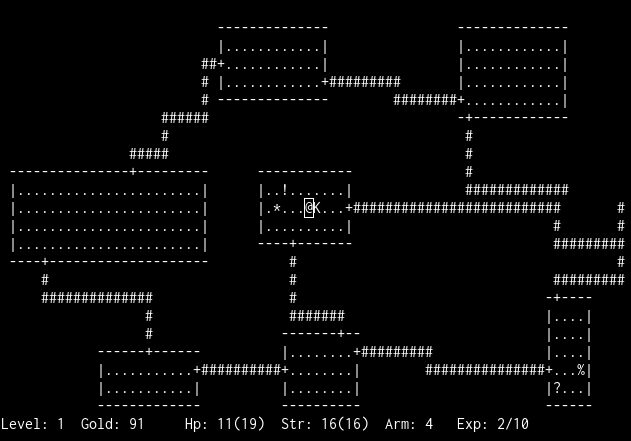
\includegraphics[scale=0.5]{rogue_screenshot}
	\label{rogsc}
\end{figure}
\subsubsection{Environment}
Every floor of the dungeon is a randomly generated level consisting of several rooms connected with corridors. Rooms sometimes generate empty, but they may also generate populated with several items or enemies. When the player starts a new run, the player is placed in dungeon level 1 with some food, a mace, basic armour, a bow and arrows. 

Rogue's environment is partially observable. The dungeon configuration is initially obscured to the player, revealing itself as the player moves around. In addition, enemies on the map will only be shown to the player if the enemy is within the player character's line of sight.

The game tracks several things that are always shown to the player:
\begin{itemize}
    \item \textbf{Level} denotes the current dungeon level.
    \item \textbf{HP} (Hit Points) represents how much damage the player can take before death. The number in brackets is the player's maximum HP.
    \item \textbf{Str} (Strength) represents how strong the player is. The number in brackets is the player's maximum strength.
    \item \textbf{Gold} is how many gold coins the player has collected.
    \item \textbf{Arm} (Armour) is the player's current armour rating. Higher is better.
    \item \textbf{Exp} shows the player's experience level and total experience points. When the player earns enough experience points, the player's experience level increases, increasing the player's maximum HP.
\end{itemize}

\subsubsection{Items}
There are a wide variety of items the player can use, such as potions, scrolls, weapons and armour. Some items need to be identified before the player knows what it will do. This can either be done by using a scroll of identify, or by blindly using or wearing the item, which may be risky. Some potions have negative effects such as the potion of poison, and rings may be ``cursed''. Cursed rings may not be removed once equipped, and they reduce the player's stats. Curses can be removed with the scroll of remove curse.

\subsubsection{Combat}
As the player navigates around the dungeon, they will encounter enemies of increasing difficulty. Enemies in the game will try to harm the player by attacking and reducing the player's HP. If the player's HP reaches 0, the player loses the game.

The player can attack enemies by moving into them. This will make the player hit the enemy with their equipped weapon. Each weapon in Rogue deals a different amount of damage, so it is important to find and equip stronger weapons.

If the player defeats an enemy, they are granted ``experience points''. When the player earns enough experience points to increase their player level, their HP and Strength increases, making them stronger.


% this can be improved Character permanent death provides a very interesting situation in the game that isn't present in many other games where you can save your progress and load previous save games. \emph{Michael Toy}, Rogue's co-creator, touched on the topic of permadeath in Roguelike Celebration 2016 in \cite{gamasutra16} by saying `We were trying to make it more immersive by making things matter ... ``this thing matters, so I'm going to think about this.'''. Every decision you make has weight to it, as the player is unable to undo any mistakes they make or adverse situations they end up in, so the player is inclined to think their actions through, providing a sense of tension in the game that would otherwise be absent.



% Rogue is a partially observable Markov Decision Process. To deal with this, we use a Long Short-term Memory system, an extension of a feedforward neural network, to process the sequence of observations. This is because LSTMs are capable of ``remembering'' information for longer periods of time. The LSTM algorithm was first defined by \cite{hochreiter97} and popularised much later, one example of an agent implementing a LSTM including AlphaStar by \cite{vinyals19}.

% The goal of chizuru4rogue is to improve upon the work of \cite{asperti18} by introducing enemies and items into the Rogue world for the agent to deal with. The agent will endeavour to maximise the final score that it gets within one run. A run's final score is used as the reward for the reinforcement learning methods within the agent. A run's final score is determined by how much gold a player collects. The deeper a player ventures in the dungeon, the more gold they can collect. Additionally, the player gains a large score bonus if the game ends while the player possesses the Amulet of Yendor, an item found in dungeon level 26.

% We use a combination of supervised learning and self-play. During the supervised learning portion of the learning process, we provide replays of Rog-o-Matic completing the game. During the self-play portion of the learning process, chizuru4rogue will play thousands of runs interfacing with Rogueinabox to receive game state and send actions.

% Using only reinforcement learning is challenging, mainly due to the large action space that Rogue provides. Unlike most other video games where the actions you can perform is contextual, Rogue is a game where every single command is available to you at all times. This allows the player to develop a wide variety of strategies, but increases the overall complexity of the game. Additionally, some commands are combined with selecting an item from the player's inventory e.g. ``wear chain mail armour'', increasing the size of the action space in different contexts.



\section{Network Architecture}
The objective of the neural network for Chizuru is to take in the observed dungeon map, player status, recent message and inventory as inputs and return an action that will maximise the expected reward as output as if it were maximising an action-value function.

Actions in Rogue are divided into basic actions and actions that utilise an inventory item, depending on the action and the item type. For example, the "eat" action can be used to make the player eat some food. If the player attempts to use an action on an item where it wouldn't make sense, a humorous message is displayed to the player such as `Ugh, you would get ill if you ate that'.

When the player uses an action that utilises an item, the game will await the player to input a key. Every item in the player's inventory maps to one key on the keyboard. The player may input \texttt{*} in order to see what legal items they may choose and their corresponding key. Additionally, the player may see what the item to keyboard mapping is by viewing their inventory with the \texttt{i} key during the game.

\subsection{Policy Optimisation}
Our goal was to find an optimal policy that maximises the chance that the agent can successfully reach the 26th dungeon level and get the Amulet of Yendor.
\subsection{State Representation}
The agent will use Rogueinabox to interface with the game. Rogueinabox is a program
\subsection{Reward Representation}
\subsection{Neural Network}

\subsection{Hyperparameters}




\section{Implementation}
\subsection{Language}
The agent will be implemented in Python. Python is one of the most popular languages used to model neural networks due to the large amount of artificial intelligence related libraries that are available for the language. The main library we will be using is TensorFlow, a library that streamlines the creation of machine learning models in Python by providing the programmer with tools to construct models, visualise data and more.


\section{Agent Training and Investigation}
\subsection{Evaluation}
During our training of the agent, we measured the agent's performance with the following criteria after every run:
\begin{itemize}
    \item The final score the agent achieved
    \item The deepest dungeon level the agent entered
\end{itemize}

\section{Conclusion and Future work}
chizuru4rogue achieves its goal on being an improvement to \cite{asperti18}'s simple navigation by being able to use items in game and fight monsters.

For future developments of the model, we plan to use *** to *** because ***

\section{Reflection}
% Write some bollocks on how RL works well on video games and how this can lead to real-world developments with this technology.

\medskip

\bibliographystyle{agsm}
\bibliography{diss}

\end{document}
